%%%%%%%%%%%%%%%%%%%%%%%%%%%%%%%%%%%%%%%%%
% Journal Article
% LaTeX Template
% Version 1.4 (15/5/16)
%
% This template has been downloaded from:
% http://www.LaTeXTemplates.com
%
% Original author:
% Frits Wenneker (http://www.howtotex.com) with extensive modifications by
% Vel (vel@LaTeXTemplates.com)
%
% License:
% CC BY-NC-SA 3.0 (http://creativecommons.org/licenses/by-nc-sa/3.0/)
%
%%%%%%%%%%%%%%%%%%%%%%%%%%%%%%%%%%%%%%%%%

%----------------------------------------------------------------------------------------
%	PACKAGES AND OTHER DOCUMENT CONFIGURATIONS
%----------------------------------------------------------------------------------------

\documentclass[twoside,twocolumn]{article}


\usepackage[
backend=biber,
style=alphabetic,
sorting=ynt
]{biblatex}

\addbibresource{main.bib}

\usepackage{url}
\usepackage{blindtext} % Package to generate dummy text throughout this template

\usepackage[sc]{mathpazo} % Use the Palatino font
\usepackage[T1]{fontenc} % Use 8-bit encoding that has 256 glyphs
\linespread{1.05} % Line spacing - Palatino needs more space between lines
\usepackage{microtype} % Slightly tweak font spacing for aesthetics

\usepackage[english]{babel} % Language hyphenation and typographical rules

\usepackage[hmarginratio=1:1,top=32mm,columnsep=20pt]{geometry} % Document margins
\usepackage[hang, small,labelfont=bf,up,textfont=it,up]{caption} % Custom captions under/above floats in tables or figures
\usepackage{booktabs} % Horizontal rules in tables

\usepackage{lettrine} % The lettrine is the first enlarged letter at the beginning of the text

\usepackage{enumitem} % Customized lists
\setlist[itemize]{noitemsep} % Make itemize lists more compact

\usepackage{abstract} % Allows abstract customization
\renewcommand{\abstractnamefont}{\normalfont\bfseries} % Set the "Abstract" text to bold
\renewcommand{\abstracttextfont}{\normalfont\small\itshape} % Set the abstract itself to small italic text

\usepackage{titlesec} % Allows customization of titles
\renewcommand\thesection{\Roman{section}} % Roman numerals for the sections
\renewcommand\thesubsection{\roman{subsection}} % roman numerals for subsections
\titleformat{\section}[block]{\large\scshape\centering}{\thesection.}{1em}{} % Change the look of the section titles
\titleformat{\subsection}[block]{\large}{\thesubsection.}{1em}{} % Change the look of the section titles

\usepackage{fancyhdr} % Headers and footers
\pagestyle{fancy} % All pages have headers and footers
\fancyhead{} % Blank out the default header
\fancyfoot{} % Blank out the default footer
\fancyhead[C]{Machine Learning Project $\bullet$ FS22} % Custom header text
\fancyfoot[RO,LE]{\thepage} % Custom footer text

\usepackage{titling} % Customizing the title section

\usepackage{hyperref}
\usepackage{graphicx} % For hyperlinks in the PDF
\usepackage{subcaption}
\usepackage{amsmath}

%----------------------------------------------------------------------------------------
%	TITLE SECTION
%----------------------------------------------------------------------------------------

\setlength{\droptitle}{-4\baselineskip} % Move the title up

\pretitle{\begin{center}\Huge\bfseries} % Article title formatting
\posttitle{\end{center}} % Article title closing formatting
\title{Machine Learning Project} % Article title
\author{%
\textsc{Benjamin Meyer}\thanks{A thank you or further information} \\[1ex] % Your name
\normalsize University of Basel \\ % Your institution
\normalsize \href{mailto:benja.meyer@unibas.ch}{benja.meyer@unibas.ch} % Your email address
%\and % Uncomment if 2 authors are required, duplicate these 4 lines if more
%\textsc{Jane Smith}\thanks{Corresponding author} \\[1ex] % Second author's name
%\normalsize University of Utah \\ % Second author's institution
%\normalsize \href{mailto:jane@smith.com}{jane@smith.com} % Second author's email address
}
\date{\today} % Leave empty to omit a date

%----------------------------------------------------------------------------------------

\begin{document}

% Print the title
\maketitle

%----------------------------------------------------------------------------------------
%	ARTICLE CONTENTS
%----------------------------------------------------------------------------------------

\section{Introduction}

In the original paper \cite{zweifel_samarin_meusburger_alewell_2021} shallow landslides in Switzerland and there causal factors are investigated.
They are using the group lasso algorithm \cite{group_lasso} for estimating coefficients over a set of causal factors (or features).
The evaluated coefficients are interpreted as an indicator of the importance for each feature to get an understanding which features drive land slides.
To get a confidence interval, different model instances of the group lasso are trained by bootstrapping the data.

In this study project we want to investigate the same data but with a bayesian statistics approach.
Rather than frequentist statistic confidence intervals we want to build bayesian statistic credible intervals.
Instead of bootstrapping the group lasso, we use the Bayesian Group Lasso algorithm \cite{bayesian_group_lasso} to approximate the distribution over the coefficients directly.
The distribution, or samples from its approximation, can then be used to get the desired credible intervals.

For the Bayesian Group Lasso the software package MBSGS \cite{MBSGS} was chosen.
Later this turned out to be a mistake, as this software package only supports Bayesian Group Lasso for normal distributed outputs and not for binomial distributed outputs.
In other words we are solving a least square regression problem rather than a log loss classification problem.
Applying linear regression on binary class labels is equivalent to the LDA algorithm, therefore we simply ignored this mistake.
Note however that all here mentioned Bayesian results are Bayesian LDA with a group selection laplace prior model rather than the originally planned Bayesian Group Lasso!

Finally during the study project a bug in the original code was found and fixed.

The rest of this document is structured as follows. First we discuss the bug found in the original code (see section \ref{sec:bug}).
Then we discuss the reproduction of parts from the original result (see section \ref{sec:reproduction}).
Next we discuss the software package used for the Bayesian Group Lasso in more details (see section \ref{sec:method}) as well as our results (see section \ref{sec:results}).
Finally, we conclude this study project (see section \ref{sec:conclusion}).

%------------------------------------------------

\section{Bug in the original paper} \label{sec:bug}

\begin{figure*}
    \centering
  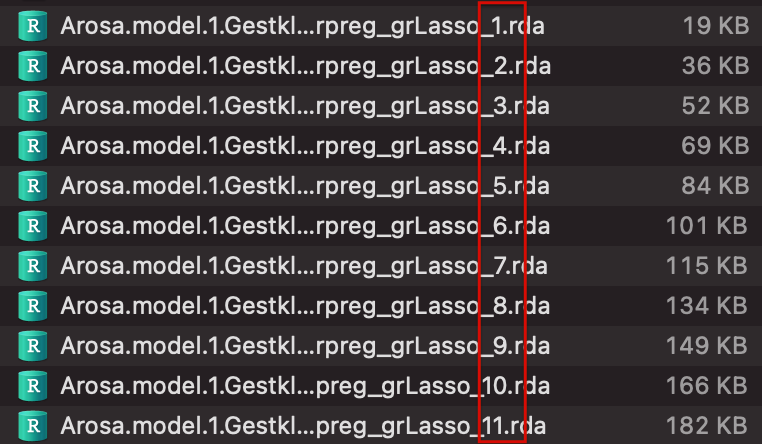
\includegraphics[width=\linewidth]{orig_filesize}
  \caption{File sizes of bootstrap run results. Red marked are the index of the bootstrap runs. We would expect that all file sizes are equal regardless of the index as all files (should) contain the result of a single bootstrap iteration.}
  \label{fig:bug_evidence}
\end{figure*}

\begin{figure*}
    \centering
    \begin{subfigure}{.33\textwidth}
      \centering
      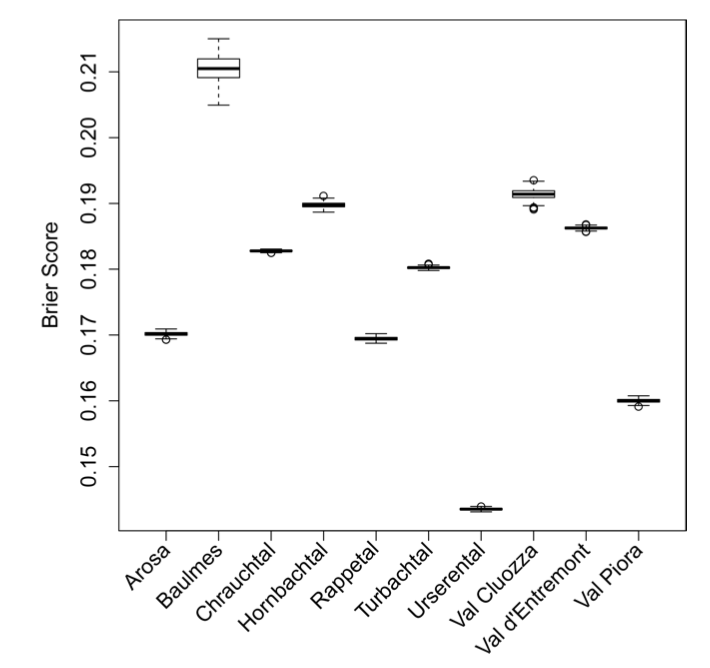
\includegraphics[width=\linewidth]{orig_brier_score}
      \caption{Original figure 9 in \cite{zweifel_samarin_meusburger_alewell_2021}}
      \label{fig:bug_fix:1}
    \end{subfigure}%
    \begin{subfigure}{.33\textwidth}
      \centering
      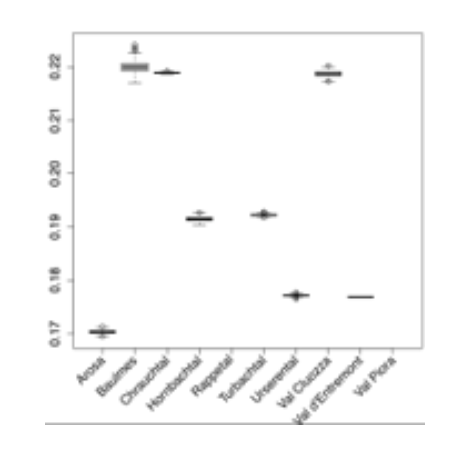
\includegraphics[width=\linewidth]{repr_brierscore_with_bug}
      \caption{Reproduction with bug}
      \label{fig:bug_fix:2}
    \end{subfigure}%
    \begin{subfigure}{.33\textwidth}
      \centering
      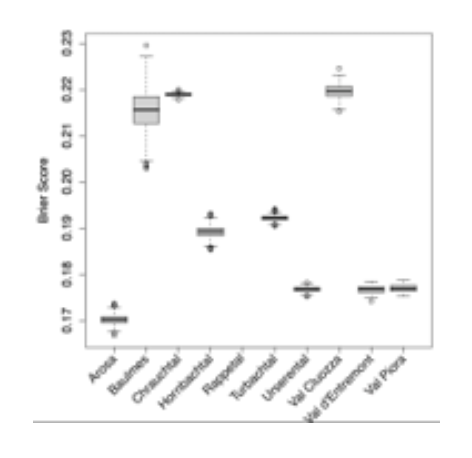
\includegraphics[width=\linewidth]{repr_brierscore}
      \caption{Reproduction with bug fix}
      \label{fig:bug_fix:3}
    \end{subfigure}
    \caption{(a) original paper (b) reproduction without bugfix. (c) reproduction with bugfix. \newline The bug caused duplication of samples therefore the confidence intervals was to narrow in the original paper. Some results differ in our reproduction (e.g Chrauchtal), the cause for this was not found. }
    \label{fig:bug_fix}
\end{figure*}

During investigating the code of \cite{zweifel_samarin_meusburger_alewell_2021}, we found a bug in accumulating the model brier score results of the bootstrap runs.
The variable for accumulating the results of the cross validation (inner loop) is not reset each bootstrap iteration (outer loop), which leads to the results of the first of $n$ bootstrap iteration being added $n$ times, the results of the second bootstrap iteration being added $n-1$ times and so on.
Therefore, some results are counted multiple times as individual results leading to a too confident confidence interval in the brier score in figure 9 in \cite{zweifel_samarin_meusburger_alewell_2021}.
The bug is quit evident when investigating the file sizes of the bootstrap runs, as shown in figure \ref{fig:bug_evidence}.

In Figure \ref{fig:bug_fix} we show the confident intervals of the brier score for each site as in the original paper, our reproduction with the bug as well as our reproduction without the bug.

The bug has no effect on the coefficient figure 7 in \cite{zweifel_samarin_meusburger_alewell_2021}, as the accumulating error was only done for the results used in figure 9.

\section{Reproducing results of original paper} \label{sec:reproduction}

\begin{figure*}

    \centering

    \begin{subfigure}[b]{\textwidth}
       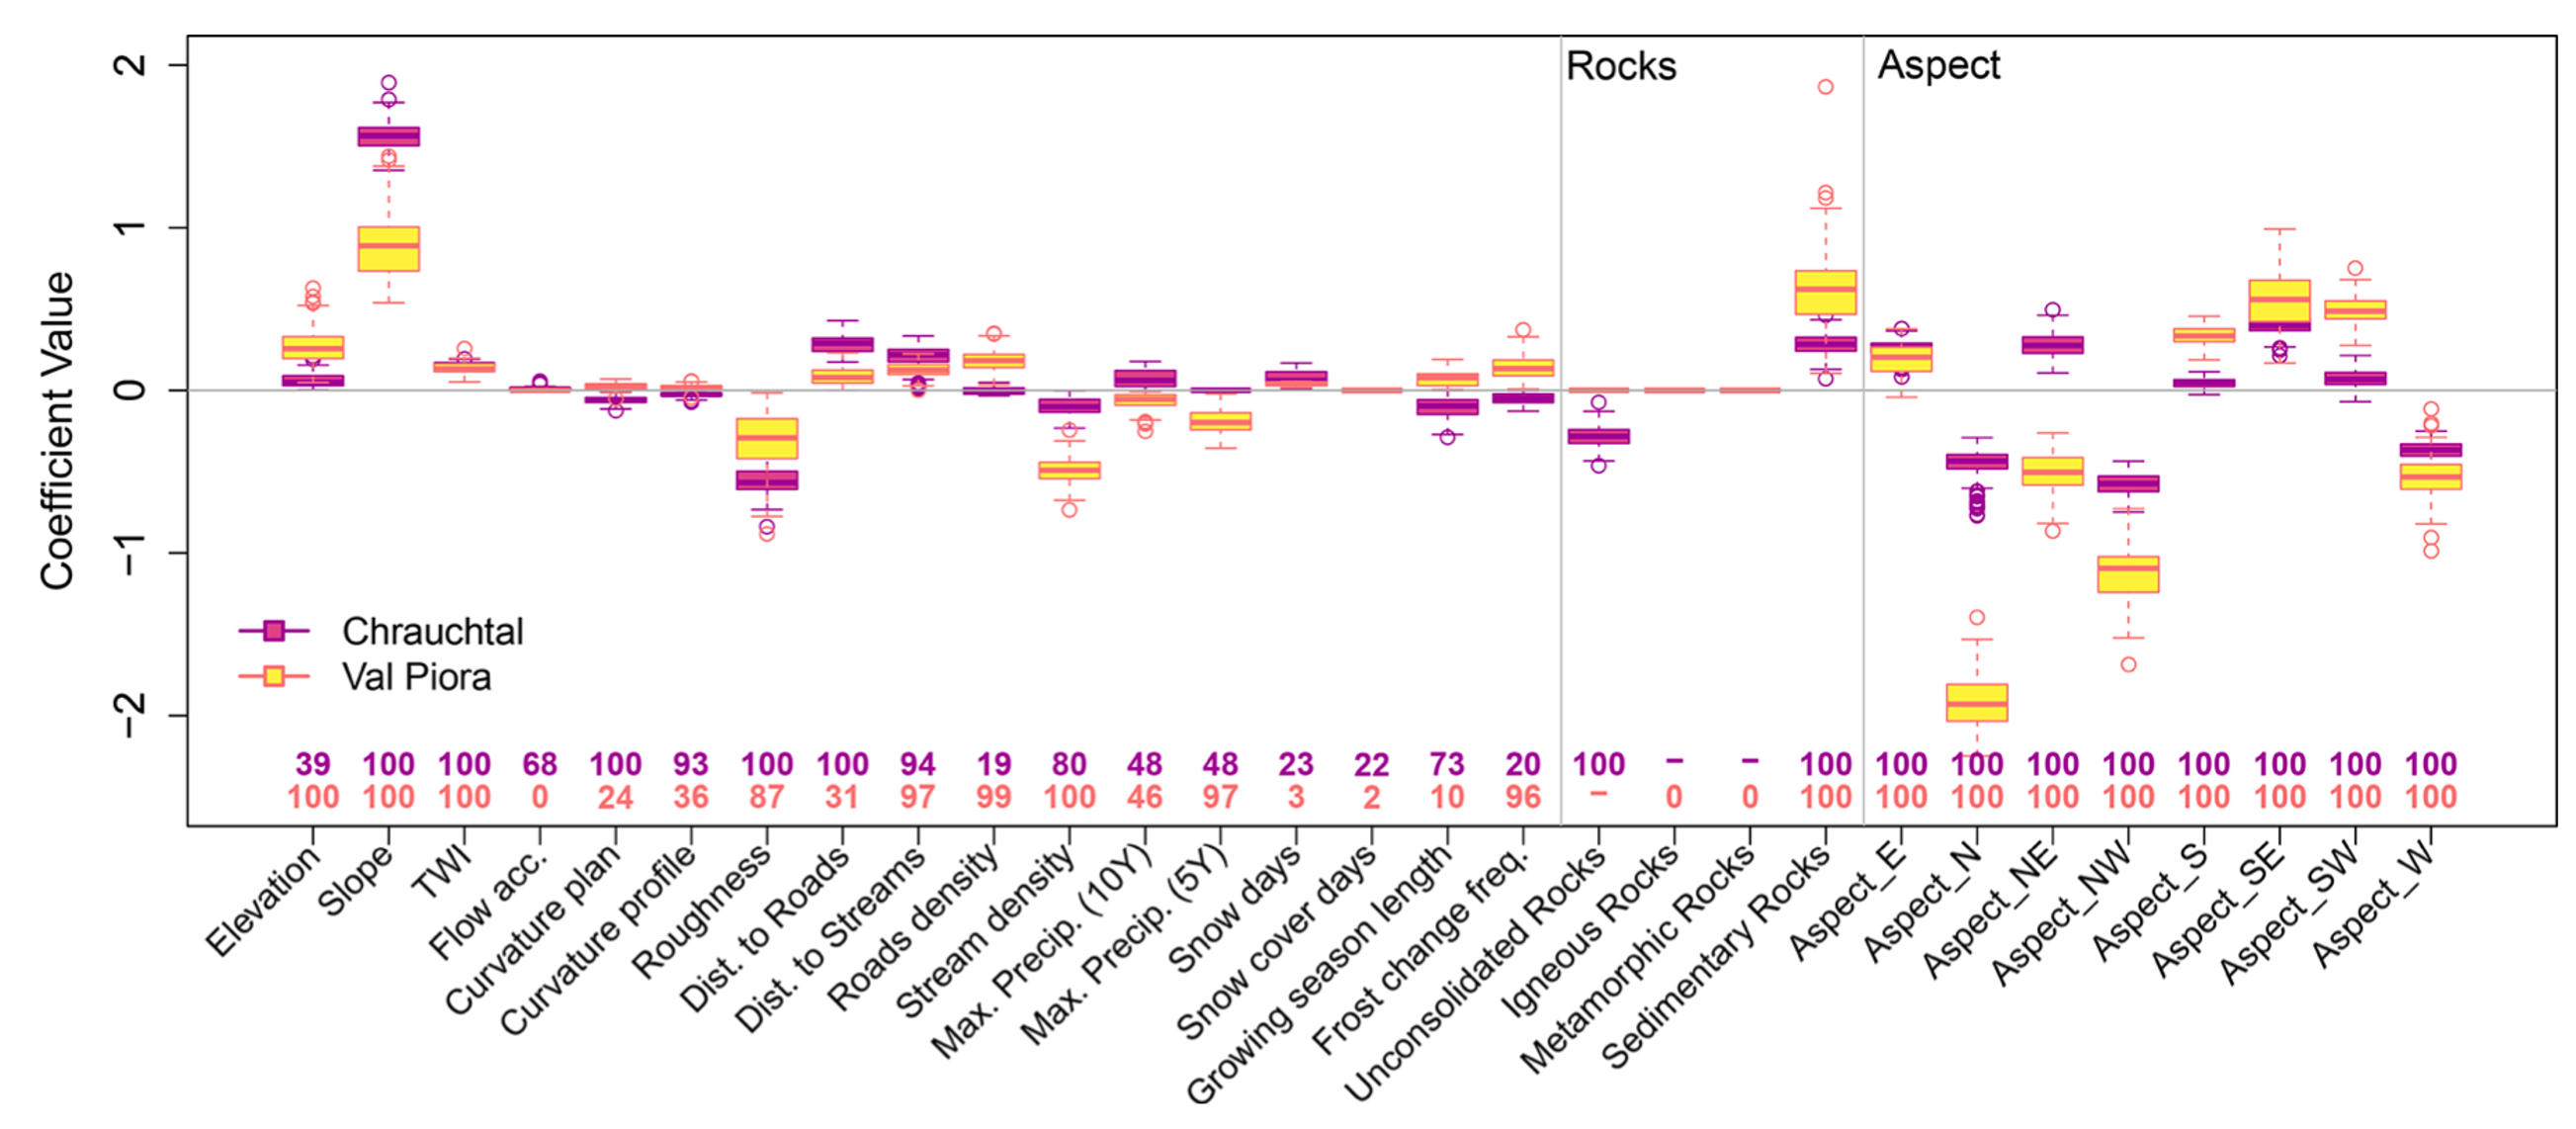
\includegraphics[width=1\textwidth]{orig_coef}
       \caption{Figure 7 from \cite{zweifel_samarin_meusburger_alewell_2021}}
       \label{fig:Ng1}
    \end{subfigure}

    \begin{subfigure}[b]{\textwidth}
       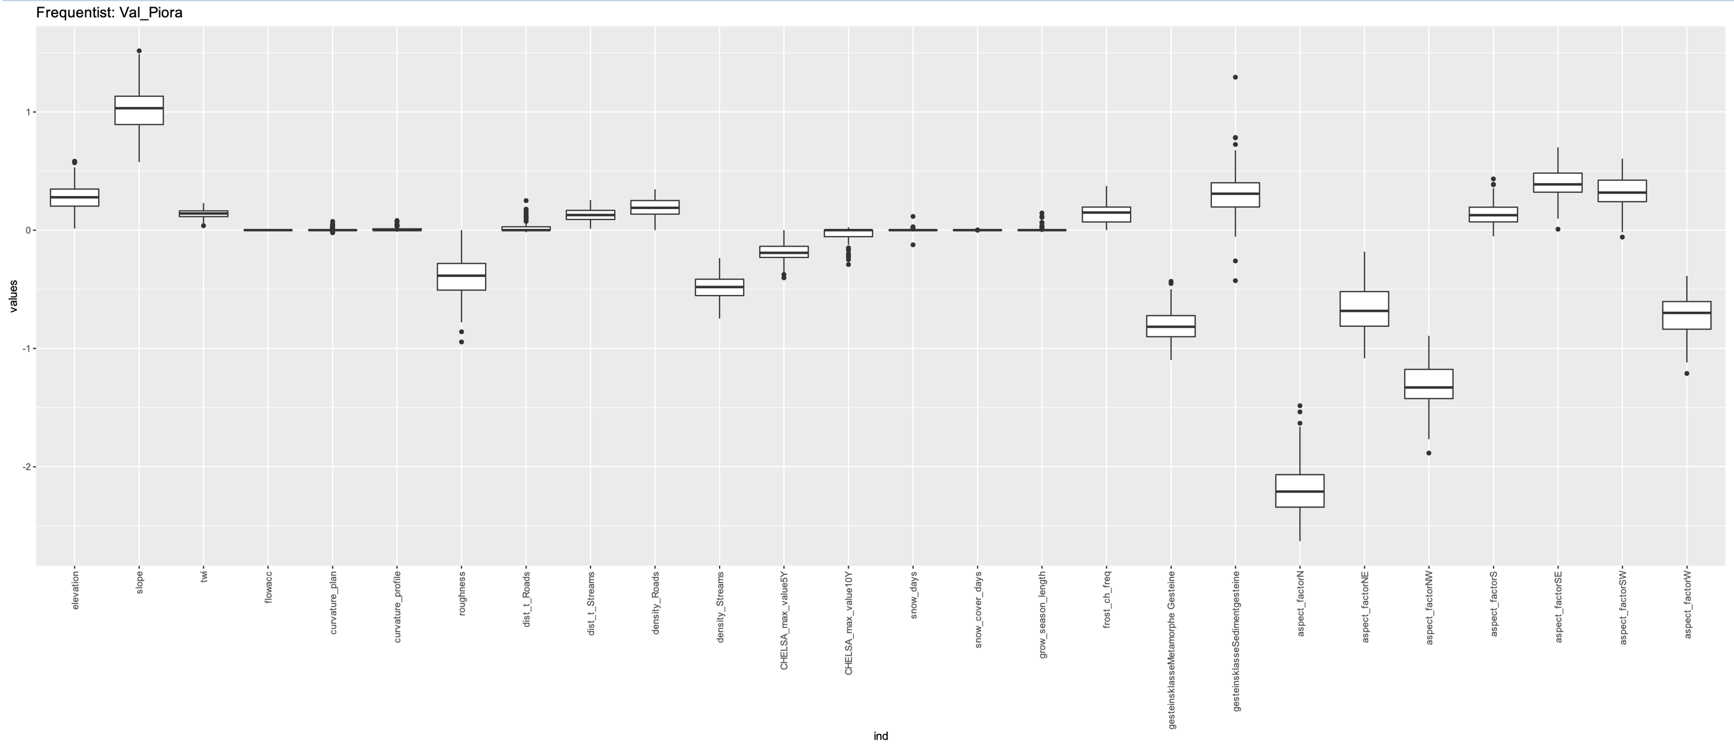
\includegraphics[width=1\textwidth]{rep_coef}
       \caption{Reproduction of coefficients from site Val Piora (yello boxplots from above figure)}
       \label{fig:Ng2}
    \end{subfigure}

    \caption[Two numerical solutions]{(a) Show the original plot from \cite{zweifel_samarin_meusburger_alewell_2021} as well as our (b) reproduction. Note that the reproduction seems to be correct. Only the categorical variables differ, which is explained as we drop the first dummy variable.}
    \label{fig:reproduction}
\end{figure*}

In figure \ref{fig:reproduction} we see the plot of the confidence intervals of the original paper as well as our reproduction.
In the reproduction the first dummy variable of each categorical feature is removed.
Otherwise, the reproduction is the same as the original paper and seems to be fine.

The reproduction was not straightforward as some used software packages had breaking changes in the meantime \cite{blockcv_issue} and the preprocessing script had to be manually edited for each site.

\section{Methods} \label{sec:method}

\subsection{Lasso}

The Lasso is a Linear Regression with a L1-Regularization on the weights.
The cost function is therefore the following:

\begin{align}
    \text{MSE}(\vec{y}, \vec{x}\vec{\beta}) + \lVert\vec{\beta}\rVert_1
\end{align}

where:

\begin{align}
    \text{MSE} & = \text{Mean Squared Error} \\
    \vec{x} & = \text{Input} \\
    \vec{\beta} & = \text{Weights} \\
    \lVert\vec{\beta}\rVert_1 & = \text{L1 Norm}
\end{align}

\subsection{Group Lasso}

The Group Lasso puts features into groups.
The idea being that features in a group are selected all together or not at all.

This is achieved by first calculating the L2 norm of the features inside a group and then calculating the L1 norm across all those group or rather L2 norms.

Note that the L2 norm has no inherit selection mechanism whereas the L1 norm does.
Therefore, we achieve what we set out to do: We select features on the group level.

Written mathematically in an unusual style where we take the norms over sets, this looks like this:

\begin{align}
    \text{MSE}(\vec{y}, \vec{x}\vec{\beta}) + \lVert \{ \lVert \beta_g \rVert_2 \mid \forall{\beta_g \in G} \} \rVert_1
\end{align}

where:

\begin{align}
    \text{G} & = \text{Partition of elements in } \beta \\
\end{align}

\subsection{Bayesian Group Lasso with Spike and Slab prior}

The Bayesian treatment of the Lasso is simply a Laplace Prior on the weights.

The Bayesian treatment of the Group Lasso is the Bayesian Group Lasso.
For the Bayesian Group Lasso the features are again grouped.

The prior per group $\beta_g$ is then simply a Multivariate Laplacian:

\begin{align}
    \pi(\beta_g) \propto \exp(-\frac{\lambda}{\sigma} \lVert \beta_g \rVert_2)
\end{align}

And the prior for the group partition $G$ is simply the product of each priors:

\begin{align}
    \pi(G) = \prod_{\beta_g in G} \pi(\beta_g)
\end{align}

To actually work with those priors, we must rewrite them in a more useful form as described in section 2 of \cite{bayesian_group_lasso}.
Rather than doing it ourselves, we use the $BGLSS$ method of the software package MBSGS \cite{MBSGS} based on \cite{bayesian_group_lasso}.

\subsection{BGLSS: Bayesian Group Lasso with Spike and Slab prior}

We are using the $BGLSS$ method of the software package MBSGS \cite{MBSGS}.
The method runs a gibbs sampler for sampling 10000 samples of the posterior distribution with a burn in phase of 5000 steps.
The regularization strength parameter is chosen by the Monte Carlo EM algorithm \cite{casella_2001}, so it must not be specified.
In the group lasso of the original paper a nested cross validation for this hyper parameter selection is run.

\section{Results} \label{sec:results}

In figure \ref{fig:results} we show the confidence and credible intervals for the site Val Piora.
It shows the confidence we have in the value of the coefficient for a particular feature.
The confidence intervals are created by the bootstrapped results, whereas the confidence intervals are created by the samples of the posterior distribution.

The credible intervals are similar to the confidence intervals.
For features that are never or not often selected in the original approach (e.g snow dasys), the new approach seems to have more outliers.
This could be due to the different regularization strength, which adds a different selection threshold.
The scale of the coefficients differ, this could be due to the different cost function used in the new approach (LDA) as well as a different regularization strength, which causes a different shrinkage behavior.

\begin{figure*}

    \centering

    \begin{subfigure}[b]{\textwidth}
       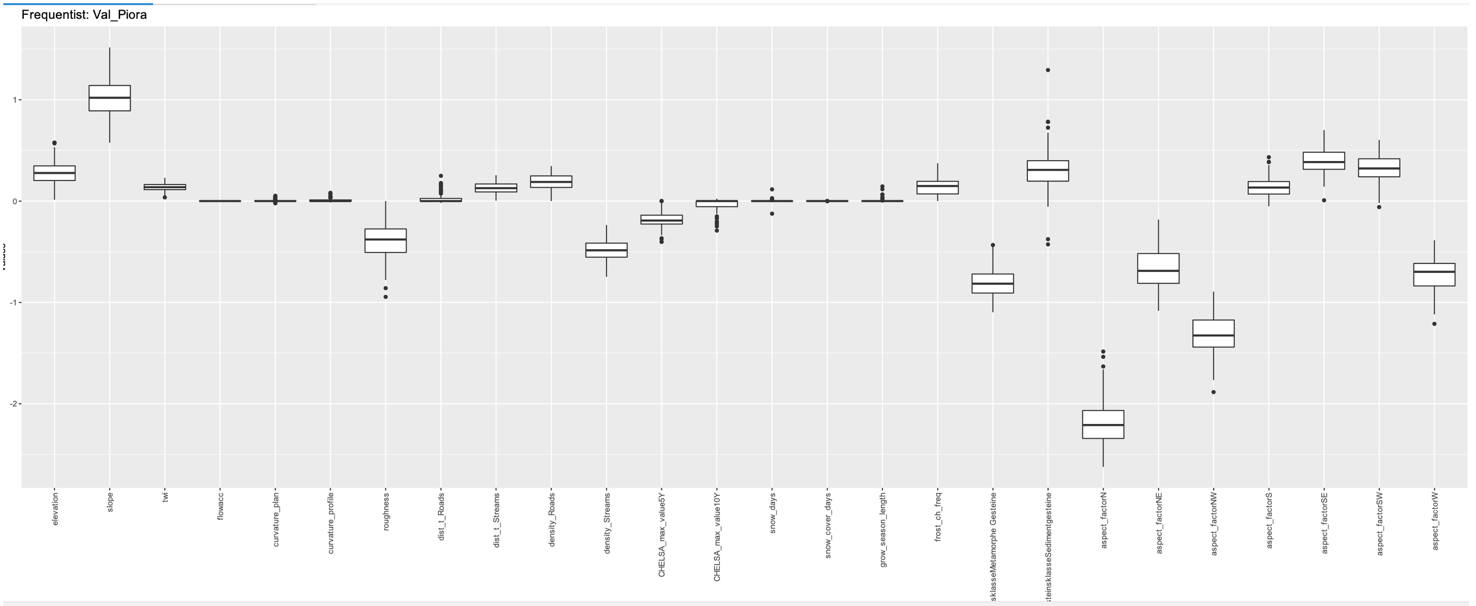
\includegraphics[width=1\textwidth]{repr_coef_result}
       \caption{Confidence interval for the coefficients at the site Val Piora with Group Lasso as well as bootstrapping}
       \label{fig:res_1}
    \end{subfigure}

    \begin{subfigure}[b]{\textwidth}
       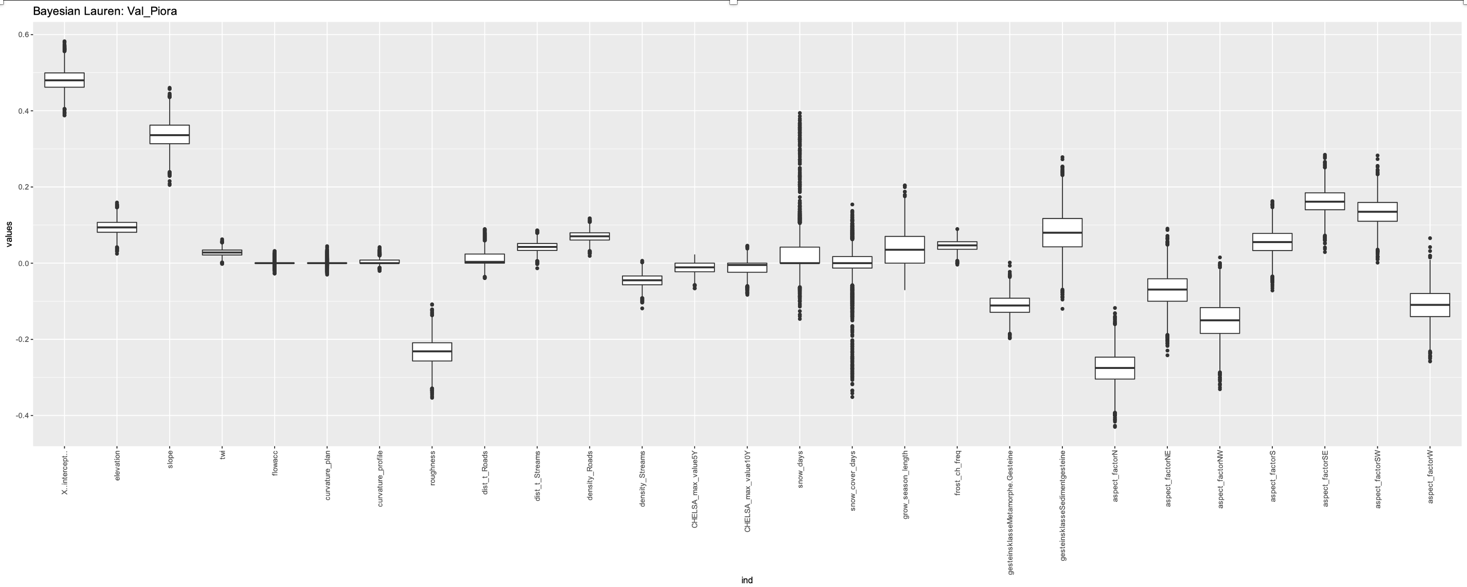
\includegraphics[width=1\textwidth]{bayes_coef_result}
       \caption{Credible intervals for the coefficients at the site Val Piora with Bayesian LDA with group selection laplace prior.}
       \label{fig:res_2}
    \end{subfigure}

    \caption{Results for the site Val Piora}
    \label{fig:results}
\end{figure*}

\section{Conclusion} \label{sec:conclusion}

I wanted to do this study project to further my understanding of the bayesian approach covered in the machine learning lecture.
In my daily work I often use frequentist models like Neural Networks or Gradient Boosting and I wanted to have a better understanding of how to use Bayesian models in practice.

In my opinion this was partly successful.
I understand the Bayesian approach better due to reading papers, using the above-mentioned software package as well as analysing the results of the model.
On the other hand the lack of in my opinion good software packages made the use of Bayesian models for me more complicated than expected.
Initially I imagined a software package for building and training Bayesian Nets, which would be, once learned, quit easy to apply to new problems (something like Tensorflow or PyTorch for Neural Networks, but for BayesNets).

I was also surprised at how much problems I had with the programming language R.
As a software engineer that is quit fluid in multiple programing languages I had a hard time picking up R and run in many problems with data types and cryptic error messages.
Driven by this frustration I even translated the hole preprocessing to Python, yet switched back to R as I did not find a implementation of the Bayesian Group Lasso in Python.

I want to thank Professor Volker Roth for the interesting technical inputs and Maxim for the guidance and pleasant communication throughout the project.

\clearpage

\printbibliography

\end{document}
